%%%%%%%%%%%%%%%%%%%%%%%%%%% asme2e.tex %%%%%%%%%%%%%%%%%%%%%%%%%%%%%%%%%
% Template for producing ASME-format articles using LaTeX            %
% Written by   Harry H. Cheng                                        %
%              Integration Engineering Laboratory                    %
%              Department of Mechanical and Aeronautical Engineering %
%              University of California                              %
%              Davis, CA 95616                                       %
%              Tel: (916) 752-5020 (office)                          %
%                   (916) 752-1028 (lab)                             %
%              Fax: (916) 752-4158                                   %
%              Email: hhcheng@ucdavis.edu                            %
%              WWW:   http://iel.ucdavis.edu/people/cheng.html       %
%              May 7, 1994                                           %
% Last change: December 5, 1998                                      %
% Use at your own risk, send complaints to /dev/null                 %
%%%%%%%%%%%%%%%%%%%%%%%%%%%%%%%%%%%%%%%%%%%%%%%%%%%%%%%%%%%%%%%%%%%%%%

%%% use two columns and ASME format
\documentclass[twocolumn,10pt]{asme2e}

%\linespread{1.8}  %%%Double space lines (remove for final draft)
\usepackage{graphicx}
\usepackage{ifthen}
\usepackage{dcolumn}% Align table columns on decimal point
\usepackage{multirow}
\usepackage{booktabs}
\usepackage{bm}% bold math
\usepackage{amsbsy}
\usepackage{amsmath}


\newcommand{\SUM}[2]{\ifthenelse{\equal{#1}{0}}{\sum_{\alpha_{#2},b_{#2},l_{#2}}^{3,n,N}} {\ifthenelse{\equal{#1}{1}}{\sum_{\alpha_{#2},b_{#2}}^{3,n}}{\sum_{\pmb{\kappa}#2,\nu#2}^{N,3n}}}}

\newcommand{\SUMprime}[2]{\ifthenelse{\equal{#1}{0}}{\sum_{\alpha_{#2},b_{#2},l_{#2}}^{3,n,N}} {\ifthenelse{\equal{#1}{1}}{\sum_{\alpha_{#2},b_{#2}}^{3,n}}{\sum_{\pmb{\kappa}^{'}#2,\nu#2}^{N,3n}}}}

\newcommand{\SUMalpha}[2]{\ifthenelse{\equal{#1}{0}}{\sum_{\alpha_{#2}}^{3}} {\ifthenelse{\equal{#1}{1}}{\sum_{\alpha_{#2},b_{#2}}^{3,n}}{\sum_{\pmb{\kappa}#2,\nu#2}^{N,3n}}}}

\newcommand{\SUMalphap}[2]{\ifthenelse{\equal{#1}{0}}{\sum_{\alpha'_{#2}}^{3}} {\ifthenelse{\equal{#1}{1}}{\sum_{\alpha'_{#2},b'_{#2}}^{3,n}}{\sum_{\pmb{\kappa}#2,\nu#2}^{N,3n}}}}

\newcommand{\SUMb}[2]{\ifthenelse{\equal{#1}{0}}{\sum_{b_{#2}}^{n}} {\ifthenelse{\equal{#1}{1}}{\sum_{\alpha_{#2},b_{#2}}^{3,n}}{\sum_{\pmb{\kappa}#2,\nu#2}^{N,3n}}}}

\newcommand{\SUMbp}[2]{\ifthenelse{\equal{#1}{0}}{\sum_{b'_{#2}}^{n}} {\ifthenelse{\equal{#1}{1}}{\sum_{\alpha'_{#2},b'_{#2}}^{3,n}}{\sum_{\pmb{\kappa}#2,\nu#2}^{N,3n}}}}

\newcommand{\SUMl}[2]{\ifthenelse{\equal{#1}{0}}{\sum_{l_{#2}}^{N}} {\ifthenelse{\equal{#1}{1}}{\sum_{\alpha_{#2},b_{#2}}^{3,n}}{\sum_{\pmb{\kappa}#2,\nu#2}^{N,3n}}}}

\newcommand{\SUMlp}[2]{\ifthenelse{\equal{#1}{0}}{\sum_{l'_{#2}}^{N}} {\ifthenelse{\equal{#1}{1}}{\sum_{\alpha'_{#2},b'_{#2}}^{3,n}}{\sum_{\pmb{\kappa}#2,\nu#2}^{N,3n}}}}

\newcommand{\EXP}[1]{\exp\mspace{-5.0mu}\left[#1\right]\mspace{-3.0mu}}

\newcommand{\abcdt}[5]{\mspace{-4.0mu}\left(\mspace{-8.0mu}\begin{smallmatrix}&\ifthenelse{\equal{#1}{}}{a}{#1}&\ifthenelse{\equal{#3}{}}{c}{#3}\\&\ifthenelse{\equal{#2}{}}{b}{#2}&\ifthenelse{\equal{#4}{}}{d}{#4}\end{smallmatrix}\mspace{-2.0mu};\ifthenelse{\equal{#5}{}}{t}{#5}\right)}

\newcommand{\abcd}[4]{\mspace{-4.0mu}\left(\mspace{-8.0mu}\begin{smallmatrix}&\ifthenelse{\equal{#1}{}}{a}{#1}&\ifthenelse{\equal{#3}{}}{c}{#3}\\&\ifthenelse{\equal{#2}{}}{b}{#2}&\ifthenelse{\equal{#4}{}}{d}{#4}\end{smallmatrix}\mspace{-3.0mu}\right)}

\newcommand{\abt}[3]{\mspace{-4.0mu}\left(\mspace{-8.0mu}\begin{smallmatrix}&\ifthenelse{\equal{#1}{}}{a}{#1} \\&\ifthenelse{\equal{#2}{}}{b}{#2}\end{smallmatrix}\mspace{-2.0mu};\ifthenelse{\equal{#3}{}}{t}{#3}\right)}

\newcommand{\ab}[2]{\mspace{-4.0mu}\left(\mspace{-8.0mu}\begin{smallmatrix}&\ifthenelse{\equal{#1}{}}{a}{#1} \\&\ifthenelse{\equal{#2}{}}{b}{#2}\end{smallmatrix}\mspace{-3.0mu}\right)}

\newcommand{\kvbat}{\mspace{-4.0mu}\left(\mspace{-8.0mu}\begin{smallmatrix} &\pmb{\kappa} &b \\ &\nu &\alpha\end{smallmatrix}\mspace{-2.0mu};t\right)}

\newcommand{\kvbatp}{\mspace{-4.0mu}\left(\mspace{-8.0mu}\begin{smallmatrix} &\pmb{\kappa} &b' \\ &\nu &\alpha'\end{smallmatrix}\mspace{-2.0mu};t\right)}

\newcommand{\kvbaw}{\mspace{-4.0mu}\left(\mspace{-8.0mu}\begin{smallmatrix} &\pmb{\kappa} &b \\ &\nu &\alpha\end{smallmatrix}\mspace{-2.0mu};\omega\right)}

\newcommand{\kvbawp}{\mspace{-4.0mu}\left(\mspace{-8.0mu}\begin{smallmatrix} &\pmb{\kappa} &b' \\ &\nu &\alpha'\end{smallmatrix}\mspace{-2.0mu};\omega\right)}

\newcommand{\kvba}{\mspace{-4.0mu}\left(\mspace{-8.0mu}\begin{smallmatrix} &\pmb{\kappa} &b \\ &\nu &\alpha\end{smallmatrix}\mspace{-3.0mu}\right)}

\newcommand{\kvbap}{\mspace{-4.0mu}\left(\mspace{-8.0mu}\begin{smallmatrix} &\pmb{\kappa} &b' \\ &\nu &\alpha'\end{smallmatrix}\mspace{-3.0mu}\right)}

\newcommand{\kpvba}{\mspace{-4.0mu}\left(\mspace{-8.0mu}\begin{smallmatrix} &\pmb{\kappa}^{'} &b \\ &\nu &\alpha\end{smallmatrix}\mspace{-3.0mu}\right)}

\newcommand{\kva}{\mspace{-4.0mu}\left(\mspace{-8.0mu}\begin{smallmatrix} &\pmb{\kappa} \\ &\nu &\alpha\end{smallmatrix}\mspace{-3.0mu}\right)}

\newcommand{\kvap}{\mspace{-4.0mu}\left(\mspace{-8.0mu}\begin{smallmatrix} &\pmb{\kappa} \\ &\nu &\alpha'\end{smallmatrix}\mspace{-3.0mu}\right)}

\newcommand{\kvb}{\mspace{-4.0mu}\left(\mspace{-8.0mu}\begin{smallmatrix} &\pmb{\kappa} &b \\ &\nu \end{smallmatrix}\mspace{-3.0mu}\right)}

\newcommand{\kvbp}{\mspace{-4.0mu}\left(\mspace{-8.0mu}\begin{smallmatrix} &\pmb{\kappa} &b' \\ &\nu \end{smallmatrix}\mspace{-3.0mu}\right)}

\newcommand{\kvt}{\mspace{-4.0mu}\left(\mspace{-8.0mu}\begin{smallmatrix}&\pmb{\kappa} \\&\nu\end{smallmatrix}\mspace{-2.0mu};t\right)}

\newcommand{\kpvt}{\mspace{-4.0mu}\left(\mspace{-8.0mu}\begin{smallmatrix}&\pmb{\kappa}^{'} \\&\nu\end{smallmatrix}\mspace{-2.0mu};t\right)}

\newcommand{\kvw}{\mspace{-4.0mu}\left(\mspace{-8.0mu}\begin{smallmatrix}&\pmb{\kappa} \\&\nu\end{smallmatrix}\mspace{-2.0mu};\omega\right)}

\newcommand{\kv}{\mspace{-4.0mu}\left(\mspace{-8.0mu}\begin{smallmatrix}&\pmb{\kappa} \\&\nu\end{smallmatrix}\mspace{-3.0mu}\right)}

\newcommand{\lbt}{\mspace{-4.0mu}\left(\mspace{-8.0mu}\begin{smallmatrix}&l \\&b\end{smallmatrix}\mspace{-2.0mu};t\right)}

\newcommand{\lbtp}{\mspace{-4.0mu}\left(\mspace{-8.0mu}\begin{smallmatrix}&l' \\&b'\end{smallmatrix}\mspace{-2.0mu};t\right)}

\newcommand{\lt}{\mspace{-4.0mu}\left(\mspace{-8.0mu}\begin{smallmatrix}&l\end{smallmatrix}\mspace{-2.0mu};t\right)}

\newcommand{\ltp}{\mspace{-4.0mu}\left(\mspace{-8.0mu}\begin{smallmatrix}&l'\end{smallmatrix}\mspace{-2.0mu};t\right)}

\newcommand{\lb}{\mspace{-4.0mu}\left(\mspace{-8.0mu}\begin{smallmatrix}&l \\&b\end{smallmatrix}\mspace{-3.0mu}\right)}

\newcommand{\lbp}{\mspace{-4.0mu}\left(\mspace{-8.0mu}\begin{smallmatrix}&l' \\&b'\end{smallmatrix}\mspace{-3.0mu}\right)}


%%% Replace here with information related to your conference
\confshortname{DRAFT MNHMT2012}
%\conffullname{the 8$^{\rm th}$ ASME-JSME Thermal Engineering Joint Conference}
\conffullname{the ASME 2012 3$^{\rm rd}$ Micro/Nanoscale Heat and Mass Transfer International Conference}

%%%%% for date in a single month, use
\confdate{3-6}
\confmonth{March}
%%%%% for date across two months, use
%\confdate{August 30-September 2}
\confyear{2012}
\confcity{Atlanta, Georgia}
\confcountry{USA}

%%% Replace DETC2010/MECH-12345 with the number supplied to you
%%% by ASME for your paper.
\papernum{MNHMT2012-75071}

\title{COMPARISON OF SPECTRAL ENERGY DENSITY METHODS FOR PREDICTING PHONON PROPERTIES}

%%% first author
\author{Jason M. Larkin\\
\textbf{Alexandre D. Massicotte}\\
\textbf{Joseph E. Turney}\\
\textbf{Alan J. H. McGaughey}\thanks{Address all correspondence to this author.}
    \affiliation{
    Department of Mechanical Engineering\\
    Carnegie Mellon University\\\emph{}
    Pittsburgh, Pennsylvania 15213-3890\\
    Email: mcgaughey@cmu.edu
    }
}

%%% second author (this is what is printed)
%%% remove the following entry for single author
%%% add more entries for multiple authors
\author{Cristina H. Amon
	\affiliation{
    Department of Mechanical Engineering\\
    Carnegie Mellon University\\
    Pittsburgh, Pennsylvania 15213-3890\\
    }
    \affiliation{
	Department of Mechanical \& Industrial Engineering\\
    University of Toronto\\
    Toronto, Ontario M5S 3G8
    }
}

\begin{document}

\maketitle

%%%%%%%%%%%%%%%%%%%%%%%%%%%%%%%%%%%%%%%%%%%%%%%%%%%%%%%%%
\begin{abstract}
\textit{To predict the thermal conductivity of a dielectric or insulating material requires the phonon frequencies and lifetimes. Techniques for predicting these quantities have been proposed based in molecular dynamics simulation and lattice dynamics calculations. Here, two expressions for the phonon spectral energy density are described and applied to two test systems: Lennard-Jones argon and Stillinger-Weber silicon. One spectral energy density expression is derived from lattice dynamics theory, while the other uses only the atomic velocities from molecular dynamics simulation. We find that while the spectral energy density using only atomic velocities can predict the phonon frequencies, it is not generally able to predict the lifetimes due to terms omitted in the derivation.}
\end{abstract}

%%%%%%%%%%%%%%%%%%%%%%%%%%%%%%%%%%%%%%%%%%%%%%%%%%%%%%%%%
%\begin{nomenclature}
%\entry{$a$}{lattice parameter}
%\subsection*{Greek}
%\entry{$\alpha$}{thermal expansion coefficient}
%\subsection*{Subscripts}
%\entry{$i$, $j$, $k$}{atomic indices}
%\end{nomenclature}


%%%%%%%%%%%%%%%%%%%%%%%%%%%%%%%%%%%%%%%%%%%%%%%%%%%%%%%%%
\section*{INTRODUCTION}

Due to the increasing prevalence of nanostructured electronic and
optoelectronic devices and the desire to employ nanostructuring to tune
material properties, it is vital to develop an understanding of the physics
of carrier transport. Phonons are the dominant energy carriers in insulators
and semiconductors, which are integral to many nanostructured devices. While
substantial effort has gone into developing adequate theories of phonon
transport, the current understanding is lacking, even in bulk materials. For
example, which phonon modes dominate energy transport and the importance of
interactions involving four or more phonons are typically unknown.  The
situation only becomes more complicated in nanostructures, where the energy
carriers also interact with surfaces and interfaces.

The usefulness of analytical models of thermal transport has been hampered by
the necessary approximations and assumptions (e.g., a Debye solid, ignoring
optical phonons), permitting only qualitative or semi-quantitative
predictions \cite{callaway1959,holland1963}. When used with the Green-Kubo or
direct methods, molecular dynamics (MD) simulations can predict thermal
conductivity \cite{mcgaughey2004c,landry2008,schelling2002,sellan2010a}.
Because the analysis in these two methods is performed at the system level,
however, no information about the phonons is obtained. The phonon properties
needed to calculate thermal conductivity (group velocities, relaxation times)
can be predicted using from harmonic and anharmonic lattice dynamics (LD)
calculations,\cite{maradudin1962,wallace1972,ladd1986,dove1993,turney2009a}
but these are theoretically and computationally complex and only valid at low
temperatures. The phonon properties can also be predicted using MD simulation and normal mode analysis
\cite{ladd1986,mcgaughey2004c,henry2008,goicochea2010} from the phonon spectral energy density (SED), which is described in the following section.

An expression for phonon SED\cite{marayuma2003,shiomi2006,dekoker2009,thomas2010c} (referred to herein as $\Phi^{'}$) has been proposed using only atomic velocities from an MD simulation as input, but has not been rigorously tested. In what follows, we derive the phonon SED from lattice dynamics
theory (referred to herein as $\Phi$). Normal mode decomposition (NMD)\cite{dove1993} is used to derive $\Phi$, which requires the phonon mode eigenvector. We then derive the alternative expression for SED $\Phi^{'}$ \cite{thomas2010c}, which does not require the phonon mode eigenvector. We demonstrate that $\Phi^{'}$ does not represent the total phonon SED while $\Phi$ does. Phonon frequencies and lifetimes are calculated and compared using $\Phi$ and $\Phi^{'}$ for two test systems: Lennard-Jones argon and Stillinger-Weber silicon. While $\Phi^{'}$ accurately predicts the phonon frequencies, it cannot predict the phonon lifetimes.  From the derivation, we show that the terms involving the phonon mode eigenvectors are responsible for the disagreement between the predicted lifetimes from $\Phi$ and $\Phi^{'}$.

\section*{THE SPECTRAL ENERGY DENSITY}\label{S:SED}

\subsection*{Derivation from Normal Mode Decomposition}\label{SS:derivation}

To derive the SED, we begin with results from standard harmonic LD theory.
The system Hamiltonian, $H$,  is\cite{turneythesis},
\begin{equation}\label{E:H_HLD}
\begin{split}
H=&\frac{1}{2}\SUM{}{}\left[\dot{q}^*\kvt \dot{q}\kvt + \omega_0^2\kv q^*\kvt q\kvt\right]\\
 =&\SUM{}{}\left[T\kvt + V\kvt\right],
 \end{split}
\end{equation}
where $t$ is time, $\omega_0\kv$ is the frequency of the phonon denoted by
wave vector $\pmb{\kappa}$ and dispersion branch $\nu$, and $N$ and $n$ are
the total number of unit cells and number of atoms in the unit cell.  The
Hamiltonian is the total system energy and is the sum of the mode- and
time-dependent kinetic and potential energies, $T\kvt$ and $V\kvt$.  The
phonon mode (normal mode) coordinate and its time derivative are given by
\begin{equation}\label{E:q_HLD}
q\kvt=\SUM{0}{}\sqrt{\frac{m_b}{N}}u_{\alpha}\lbt e^*\kvba\EXP{i\pmb{\kappa}\cdot\mathbf{r}_0\ab{l}{0}}
\end{equation}
and
\begin{equation}\label{E:qdot_HLD}
\dot{q}\kvt{}{}{}=\SUM{0}{}\sqrt{\frac{m_b}{N}}\dot{u}_{\alpha}\lbt e^*\kvba\EXP{i\pmb{\kappa}\cdot\mathbf{r}_0\ab{l}{0}},
\end{equation}
where $m_b$ is the mass of the $b^{\textrm{th}}$ atom in the unit cell, and
$\mathbf{r}_0\ab{l}{0}$ is the equilibrium position vector of the
$l^{\textrm{th}}$ unit cell. The $\alpha$-component of the displacement (from
equilibrium), $u_{\alpha}\lbt$, and velocity, $\dot{u}_{\alpha}\lbt$, of the
$b^{\textrm{th}}$ atom in the $l^{\textrm{th}}$ unit cell are time-dependent
and are related to the phonon mode coordinates through the time-independent
polarization vector $e\kvba$. The asterisk superscript in Eqs$.$
\eqref{E:q_HLD} and \eqref{E:qdot_HLD} denotes the complex conjugate.

In an anharmonic system, the phonon populations fluctuate about the
equilibrium distribution function \cite{wallace1972}. The phonon mode coordinates and their time
derivatives are
\begin{equation}\label{E:q_A}
q_A\kvt=\left[q_{SS}\kvt+q_{T}\kvt\right]
\end{equation}
and
\begin{equation}\label{E:qdot_A}
\dot{q}_A\kvt=\left[\dot{q}_{SS}\kvt+\dot{q}_{T}\kvt\right].
\end{equation}
The steady-state and transient parts and their time derivatives are given by
\begin{equation}\label{E:q_A_SS}
q_{SS}\kvt=C_1\kv\exp\lbrace i\omega_0\kv t\rbrace+C_2\kv\exp\lbrace -i\omega_0\kv t\rbrace,
\end{equation}
\begin{equation}\label{E:q_A_T}
q_{T}\kvt=\EXP{-\Gamma\kv |t|}\lbrace C_3\kv\EXP{i\omega_0\kv t}-C_4\kv\EXP{-i\omega_0\kv t}\rbrace,
\end{equation}
\begin{equation}\label{E:qdot_A_SS}
\dot{q}_{SS}\kvt=i\omega_0\kv\left\{C_1\kv\exp[i\omega_0\kv t]-C_2\kv\exp[-i\omega_0\kv t]\right\},
\end{equation}
and
\begin{multline}\label{E:qdot_A_T}
\dot{q}_{T}\kvt=\EXP{-\Gamma\kv |t|}\left\{C_3\kv\left[i\omega_0\kv-\Gamma\kv\right]\EXP{i\omega_0\kv t}\right.
\\\left.-C_4\kv\left[i\omega_0\kv+\Gamma\kv\right]\EXP{-i\omega_0\kv t}\right\},
\end{multline}
where the $C$s are constants and $\omega_0\kv$ and $\Gamma\kv$ are the phonon
mode frequency and scattering rate (i$.$e$.$, linewidth).  The transient part
describes the creation of an excess in the population of a phonon mode for
$t<0$ and its decay back to equilibrium for $t>0$.

The model used for anharmonic lattice dynamics is an excitation and decay of
a single phonon mode \cite{wallace1972}.  In a real system, there will be multiple phonons in
each mode that simultaneously grow or decay with time.  Thus, (dealing only
with $\dot{q}$) we let
\begin{multline}\label{E:qdot_A_kvbat}
\dot{q}\kvt=\sum_j i\EXP{-\Gamma\kv |t-t_j|}\\
\times\lbrace A_j\kv\left[\omega_0\kv+i\Gamma\kv\right]\EXP{i\omega_0\kv (t-t_j)}
\\-B_j\kv \left[\omega_0\kv-i\Gamma\kv\right]\EXP{-i\omega_0\kv (t-t_j)}\rbrace,
\end{multline}
where many phonons in each mode, indexed by $j$, are simultaneously being
created and destroyed.  The phonons grow for $t<t_j$ and decay for $t>t_j$
and $A_j$ and $B_j$ are constants.  We are  not concerned with the values of
$t_j$, $A_j$, and $B_j$, though they should take on values such that
$\langle\dot{q}_{SS}^*\kvt\dot{q}_{SS}\kvt\rangle=\langle\dot{q}^*\kvt\dot{q}\kvt\rangle$.

The kinetic energy of the crystal is
\begin{equation}\label{E:ave_T_t}
T\kvt=\frac{1}{2}\lim_{\tau_0\rightarrow\infty}\frac{1}{2\tau_0}\int_{-\tau_0}^{\tau_0}\dot{q}^*\kvt\dot{q}\kvt dt.
\end{equation}
The kinetic energy can be transformed from the time domain ($t$) to the
frequency domain ($\omega$) by Parseval's theorem\cite{rudin1987},  allowing
Eq$.$ \eqref{E:ave_T_t} to be written as
\begin{equation}\label{E:ave_T_w1}
T\kvw=\lim_{\tau_0\rightarrow\infty}\frac{1}{4\tau_0}\left|\frac{1}{\sqrt{2\pi}}\int_{-\tau_0}^{\tau_0}\dot{q}\kvt\exp(-i\omega t)dt\right|^2.
\end{equation}
By substituting Eq$.$ \eqref{E:qdot_A_kvbat} into Eq$.$ \eqref{E:ave_T_w1} and performing the integration over time we find
\begin{multline}\label{E:ave_T_w_int}
T\kvw=\frac{1}{16\pi\tau_0}\left|\sum_j\EXP{-i\omega t_j}\left\{A_j\kv\frac{\omega_0\kv+i\Gamma\kv}{\omega_0\kv-\omega+i\Gamma\kv}\right.\right.\\
\left.\left.+B_j\kv\frac{\omega_0\kv-i\Gamma\kv}{\omega_0\kv+\omega-i\Gamma\kv}\right\}\right|^2.
\end{multline}
We are primarily interested in values of $\omega$ where $\omega\approx\omega_0$.  When $\omega\approx\omega_0$, the term involving $A_j$ becomes large since $\Gamma<<\omega_0$ and the term involving $B_j$ can be neglected.  (Alternatively, we could ignore the term involving $A_j$ when $\omega\approx-\omega_0$.)  Hence, we find
\begin{multline}\label{E:ave_T_w_approx}
T\kvw=\frac{1}{16\pi\tau_0}\sum_j\sum_{j'}\cos\left[\omega (t_{j'}-t_j)\right]A_j\kv A_{j'}\kv\\
\times\frac{\omega_0^2\kv+\Gamma^2\kv}{\Gamma\kv}\frac{\Gamma\kv}{[\omega_0\kv-\omega]^2+\Gamma^2\kv}.
\end{multline}
We finally arrive at the expression for the phonon spectral energy density
\begin{equation}\label{E:Lorentzian_NMD}
\Phi(\omega,\pmb{\kappa})=2\sum_{\nu}^{3n}\langle T\kvw\rangle=\sum_{\nu}^{3n}C_0\kv\frac{\Gamma\kv/\pi}{[\omega_0\kv-\omega]^2+\Gamma^2\kv},
\end{equation}
where the factor of 2 comes from equipartition of kinetic and potential energy, and
\begin{equation}\label{E:C_0}
C_0\kv=\sum_j\sum_{j'}\cos\left[\omega (t_{j'}-t_j)\right]A_j\kv A_{j'}\kv\frac{\omega_0^2\kv+\Gamma^2\kv}{8\tau_0\Gamma\kv}.
\end{equation}
Thus, the phonon spectral energy $\Phi(\omega,\pmb{\kappa})$ is a superposition of $3n$ Lorentzian
functions with centers at $\omega_0\kv$ with a half-width at half-maximum of
$\Gamma\kv$. To calculate $\Phi$ one uses Eq$.$ \eqref{E:ave_T_w1}. The allowed wavevectors are determined by the crystal structure and the atomic velocities are supplied by MD simulation. $\Phi$ also requires the phonon mode eigenvectors which can be determined {\em a priori} using quasi-harmonic lattice dynamics (QHLD) calculations, which uses the temperature-dependent zero-pressure lattice constant.\cite{mcgaughey2006b} The advantage of Eq$.$ \eqref{Lorentzian_SED} is other than the wavevectors, which can be determined from the system geometry, no phonon
properties need to be known {\em a priori}.

This derivation of the phonon SED is well-defined theoretically \cite{wallace1972}. The Hamiltonian can be written as
\begin{equation}\label{E:equipartition}
H=\sum_{\pmb{\kappa}}^{N}\int_{-\infty}^{\infty}\Phi(\omega,\pmb{\kappa})d\omega=2\sum_{\pmb{\kappa},\nu}^{N,3n}\sum_{\alpha,b}^{3,n}\langle T\kvbat\rangle.
\end{equation}
We know from anharmonic LD that \cite{maradudin1962,ladd1986}
\begin{equation}\label{E:lifetime}
\tau\kv=\frac{1}{2\Gamma\kv},
\end{equation}
where $\tau$ is the phonon lifetime. Typically, anharmonic LD calculations are limited to 3-phonon scattering events, which is only a good assumption at low temperatures.\cite{turney2009a,esfarjani2011} All order phonon processes are possible in MD simulation as the atoms are evolved dynamically using the full anharmonicity of the interatomic interactions.\cite{mcgaughey2004c,landry2008,schelling2002} Thus, the lifetimes predicted by Eq$.$ \eqref{E:Lorentzian_NMD} include the effect of n-phonon scattering events.

As temperature increases, n-phonon events start to occur naturally in MD because the full anharmonic interatomic interactions are used. The normal mode decomposition method [Eq$.$ \eqref{E:Lorentzian_NMD}] does lose accuracy
at higher temperatures because the quasi-harmonic phonon frequencies and
eigenvectors are used to perform the energy mapping
\cite{turney2009a}. A comparison between LD (anharmonic LD, normal mode decomposition) and MD (non-equilibrium direct-MD, equilibrium Green-Kubo) for LJ argon shows that LD techniques start to diverge from the MD results for the thermal conductivity above half the melting temperature.  In this paper, we limit the temperature to below half the melt temperature of both Lennard-Jones argon and Stillinger Weber silicon. In this work, we are not testing the effects of n-phonon scattering events but rather are showing that $\Phi'$ is an incorrect phonon SED by comparing it directly to $\Phi$.

Once the frequencies and relaxation times of all phonon modes in the
Brillouin zone are obtained, the bulk thermal conductivity in direction
$\mathbf{n}$, $k_{\mathbf{n}}$, can be calculated from
\begin{equation}
	\label{E-size:k_bulk}
	k_{\mathbf{n}}=\sum_{\pmb{\kappa}} \sum_\nu c \kv v^{2}_{g,\mathbf{n}} \kv \tau \kv.
\end{equation}
Here, $c$ is the phonon volumetric specific heat and ${v}_{g,\mathbf{n}}$ is
the component of the group velocity vector in direction $\mathbf{n}$. Since the systems we consider are classical, the
specific heat takes on the value of $k_B$ per mode in the harmonic limit. The group
velocity vector is the gradient of the dispersion curves (i.e., $\partial
\omega /
\partial \pmb{\kappa}$), which can be calculated using finite difference and thus also requires the frequencies.

\subsection*{Proposed Alternative Formulation for Phonon Spectral Energy}\label{S:Properties}

Alternatively, one could start with the real space atomic velocities as represented by the normal mode decomposition \cite{dove1993}
\begin{equation}\label{E:udot_HLD}
\dot{u}_{\alpha}\lbt =  \SUMprime{2}{} \frac{1}{\sqrt{m_bN}} \EXP{i\pmb{\kappa}^{'}\cdot\mathbf{r}_0\ab{l}{0}} e^*\kpvba \dot{q}\kpvt{}{}{}.
\end{equation}
Fourier transforming both sides in time and space, then summing over atoms in the unit cell and Cartesian directions yields
\begin{multline}\label{SED}
\sum_\alpha^3 \sum_b^n m_b \left| \sum_l^N  \int_{-\infty}^{\infty} \dot{u}_{\alpha}\lbt \EXP{i\pmb{\kappa}\cdot\mathbf{r}_0\ab{l}{0}-i\omega t} dt \right|^2 =
\\ \sum_\alpha^3 \sum_b^n\left| \frac{m_b^{3/2}}{\sqrt{N}} \sum_l^N \sum_{\nu}^{3n} e^*\kvba \int_{-\infty}^{\infty}\dot{q}\kvt\EXP{i\pmb{\kappa}\cdot\mathbf{r}_0\ab{l}{0}-i\omega t}dt\right|^2 ,
\end{multline}
where the the sum over $\pmb{\kappa}^{'}$ is reduced to a single $\pmb{\kappa}$ by orthogonality of the allowed wavevectors. Thomas et al. \cite{thomas2010c} define
\begin{multline}\label{Lorentzian_SED}
\Phi^{'}(\omega,\pmb{\kappa}) =
\\ \frac{1}{4\pi\tau_0N} \sum_\alpha^3 \sum_b^n m_b \left| \sum_l^N  \int_{-\tau_0}^{\tau_0} \dot{u}_{\alpha}\lbt \EXP{i\pmb{\kappa}\cdot\mathbf{r}_0\ab{l}{0}-i\omega t} dt \right|^2
\end{multline}
which is the finite integration of the left side of Eq$.$ \eqref{SED}. The relation of Eq$.$ \eqref{Lorentzian_SED} to Eq$.$ \eqref{E:Lorentzian_NMD} is unclear and will be investigated in the next section. To evaluate Eq$.$ \eqref{E:Lorentzian_NMD} one uses Eq$.$ \eqref{E:ave_T_w1}.

\subsection*{PHONON PROPERTIES FROM SPECTRAL ENERGY}\label{S:Properties}

\section*{Lennard-Jones Argon Case Study}\label{S:LJ_Case_study}

We now use molecular dynamics (MD) simulation to compare the spectral energy calculated for Lennard-Jones argon \cite{mcgaughey2004c} using Eqs$.$ \eqref{E:ave_T_w1} and \eqref{Lorentzian_SED}. We consider temperatures of 5,20, and 40 K at zero-pressure.  The MD system consists
of $8\times 8\times 8$ conventional unit cells ($b=4$ atoms) for a total of 2048 atoms.
Using a 4.285 fs time step, the system is equilibrated for $2^{20}$ time steps before collecting data every $2^5$ time step for an additional $2^{20}$ time steps. The calculations performed here are averaged from five independent simulations (with different initial conditions).

The spectral energy [Eqs$.$ \eqref{E:ave_T_w1} and \eqref{Lorentzian_SED}] for a wavevector in the [100] direction with magnitude $\pi/2a$ is presented in Fig$.$ \ref{F:PEAK_COMPARE}. For Eq$.$ \eqref{E:ave_T_w1} the spectral curve is plotted as a superposition over the different phonon polarizations $\nu$.  Overall, we see that the spectral energy Eq$.$ \eqref{Lorentzian_SED} does not equal the total phonon spectral energy Eq$.$ \eqref{E:ave_T_w1}, but the spectral features are very similar to with peaks shifted in magnitude. It is worth noting that the linewidth (inverse lifetime) defined in Eq$.$ \eqref{E:ave_T_w1} is independent of the Lorentzian peak magnitude. The linewidths at $5$ and $20$K look similar between the two spectral curves. However, as the temperature increases to $40$K, there are clear linewdith variations between the two spectral curves. These linewidth variations translate to variations in the predicted phonon lifetimes by Eq \eqref{E:lifetime}.

The phonon frequencies and lifetimes have been extracted for all allowed wavectors in the first Brioullin zone (BZ) of the cubic conventional cell using both expressions for the spectral energy. This is done by fitting the spectral peaks with Lorentzian functions using a non-linear least squares method. For $\Phi'$, the SED for different polarizations at a given wavevector are superimposed by definition of Eq$.$ \ref{Lorentzian_SED}. For $\Phi$ or $\Phi'$, the different polarizations can each be fit individually using single Lorentzian peaks or simultaneously as a superposition of peaks. At the temperatures studied in this work, we find that the difference between fitting single or simultaneous peaks is less than 5 percent. The error in fitting the Lorentzian functions is between $5-10\%$, with the error increasing with temperature.

The measured frequencies $\omega\kv$ and lifetimes $\tau\kv$ are compared on a mode-by-mode basis in Fig$.$ \ref{F:FREQ_LIFE_LJ}. Here $\omega$, $\omega^{'}$ and $\tau$, $\tau^{'}$  refer to mode properties measured using Eqs$.$ \eqref{E:ave_T_w1} and \eqref{Lorentzian_SED}. The phonon frequencies agree well for all three temperatures, with increasing scatter at high temperatures.  This is because the spectral curves in Eq$.$ \eqref{Lorentzian_SED} are a superposition over the different phonon polarizations $\nu$, while the spectral curves can be isolated for individual polarizations in Eq$.$ \eqref{E:ave_T_w1}. At high temperature and frequency the broadening superposition of polarizations make it difficult to locate the peaks in Eq$.$ \eqref{Lorentzian_SED}. While the phonon frequencies can be predicted accurately by Eqs$.$ \eqref{Lorentzian_SED}, the lifetimes show large scatter on a mode-by-mode basis, with increasing scatter at high temperature.  This can be attributed to the undetermined factors involving the phonon mode eigenvectors in Eq$.$ \eqref{Lorentzian_SED} and is examined in a following section.

\begin{figure}
\begin{center}
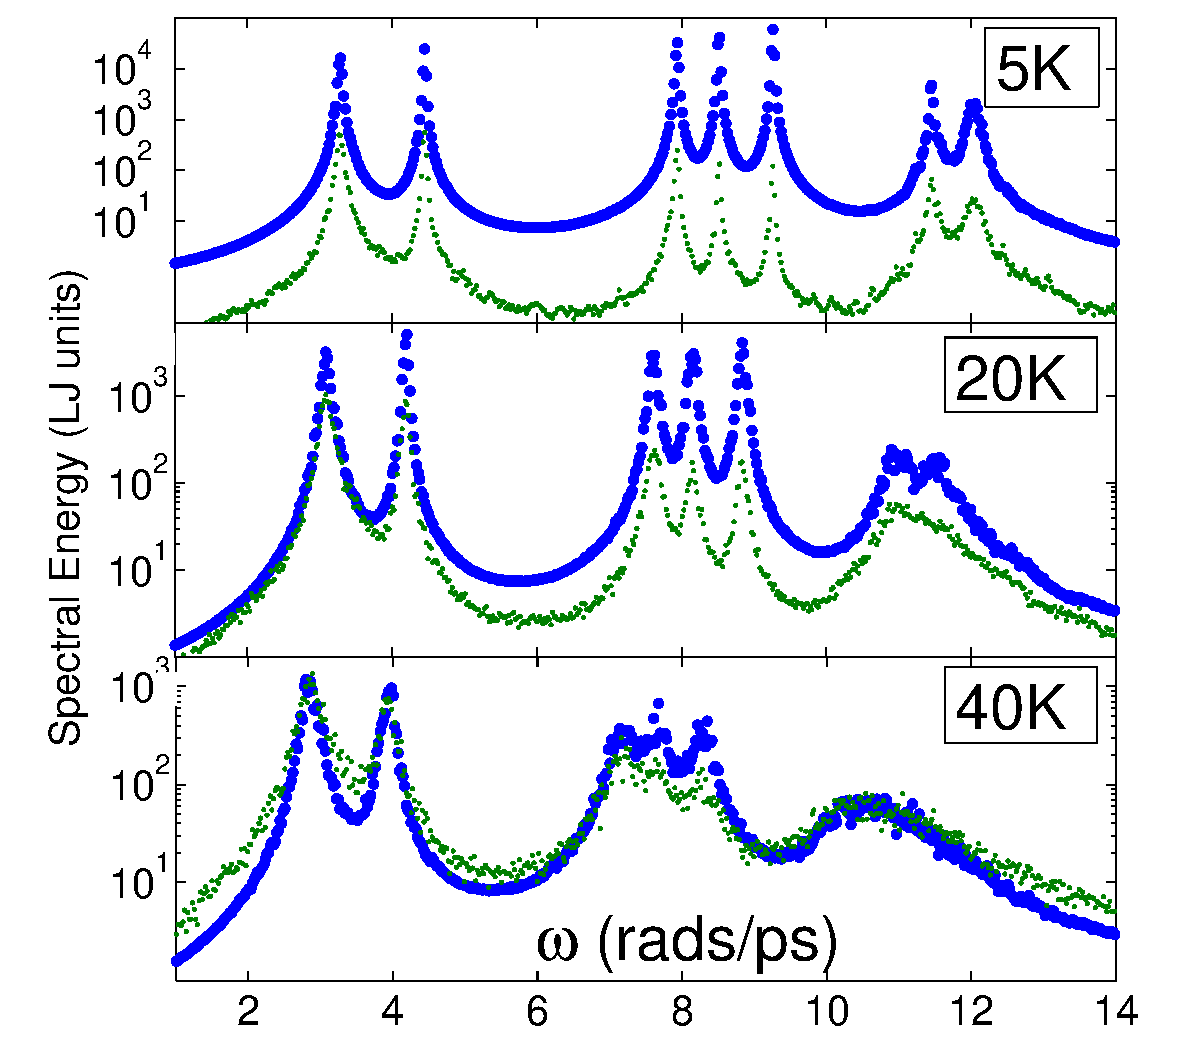
\includegraphics[angle=0,width=90.0mm]{LJ_NMD_SED_PEAK_COMPARE.eps}
\end{center}
\caption{\label{F:PEAK_COMPARE} THE TOTAL PHONON SPECTRAL ENERGY [EQ$.$ \eqref{E:ave_T_w1}] IS PLOTTED IN LARGE CIRCLES.  THE SPECTRAL ENERGY IN EQ$.$ \eqref{Lorentzian_SED} IS PLOTTED IN SMALL POINTS. THE WAVEVECTOR IS IN THE [100] DIRECTION WITH MAGNITUDE $\pi/2a$.}
\vspace*{-5mm}
\end{figure}

\begin{figure}
\begin{center}
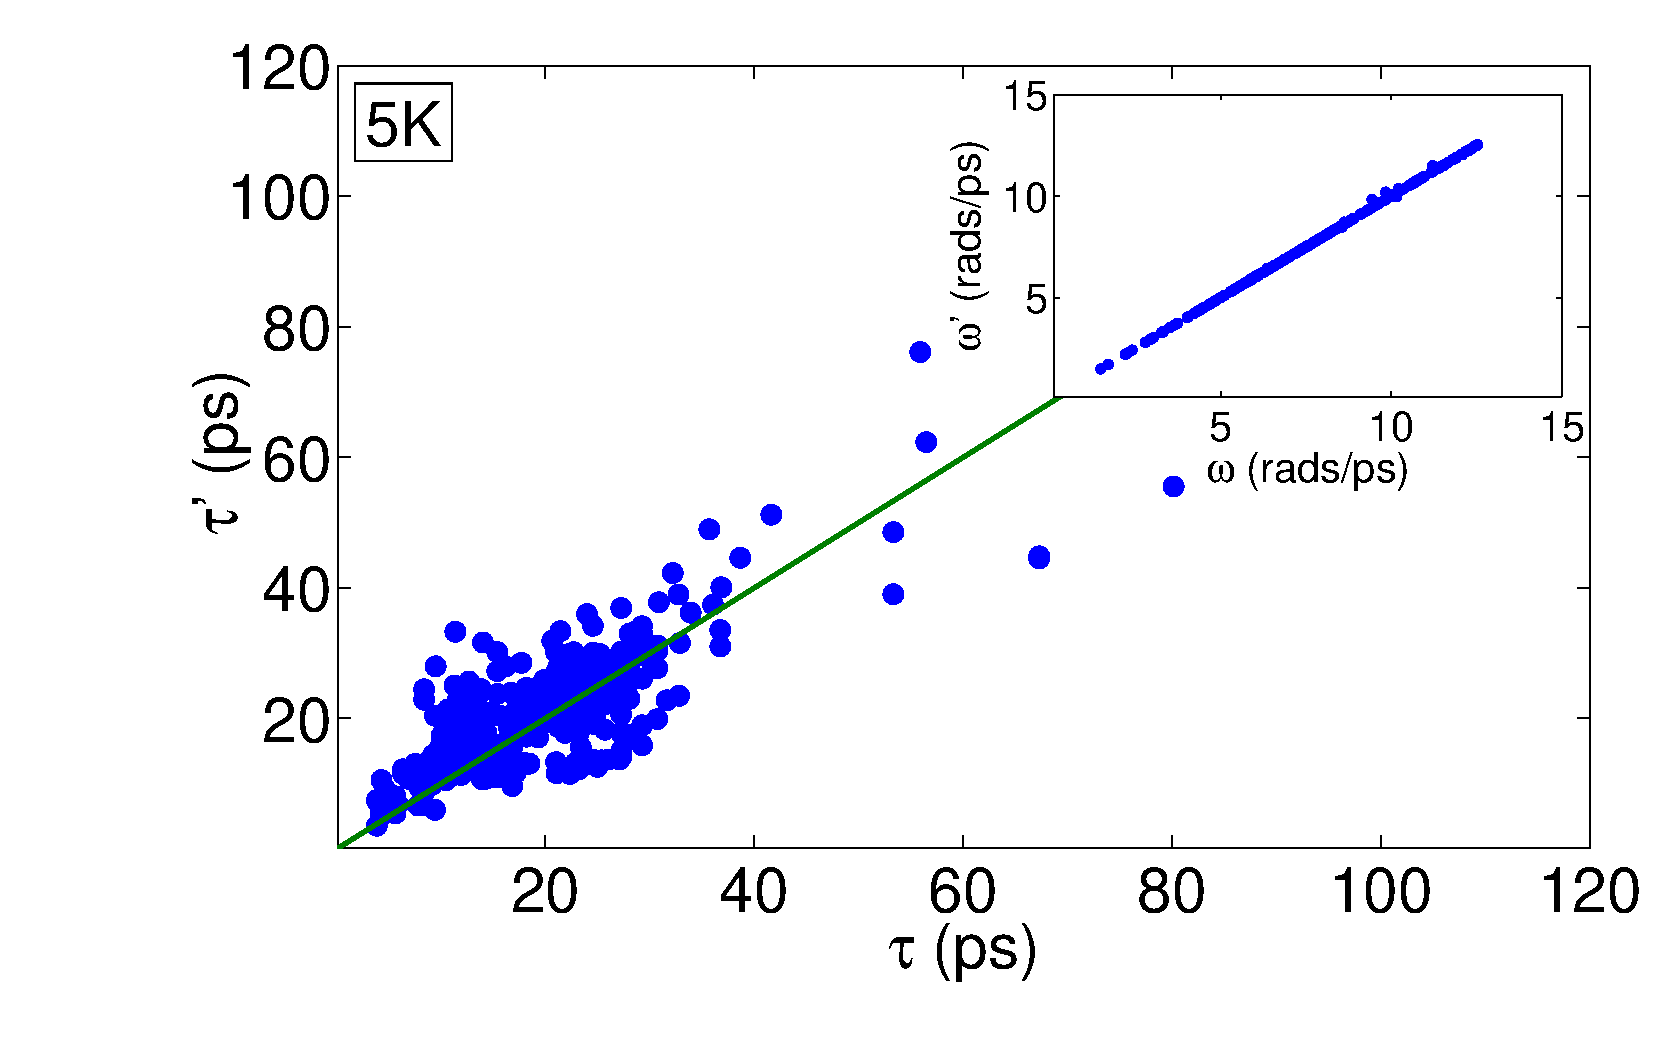
\includegraphics[angle=0,width=80.0mm]{LJ_NMD_SED_5K_2.eps}
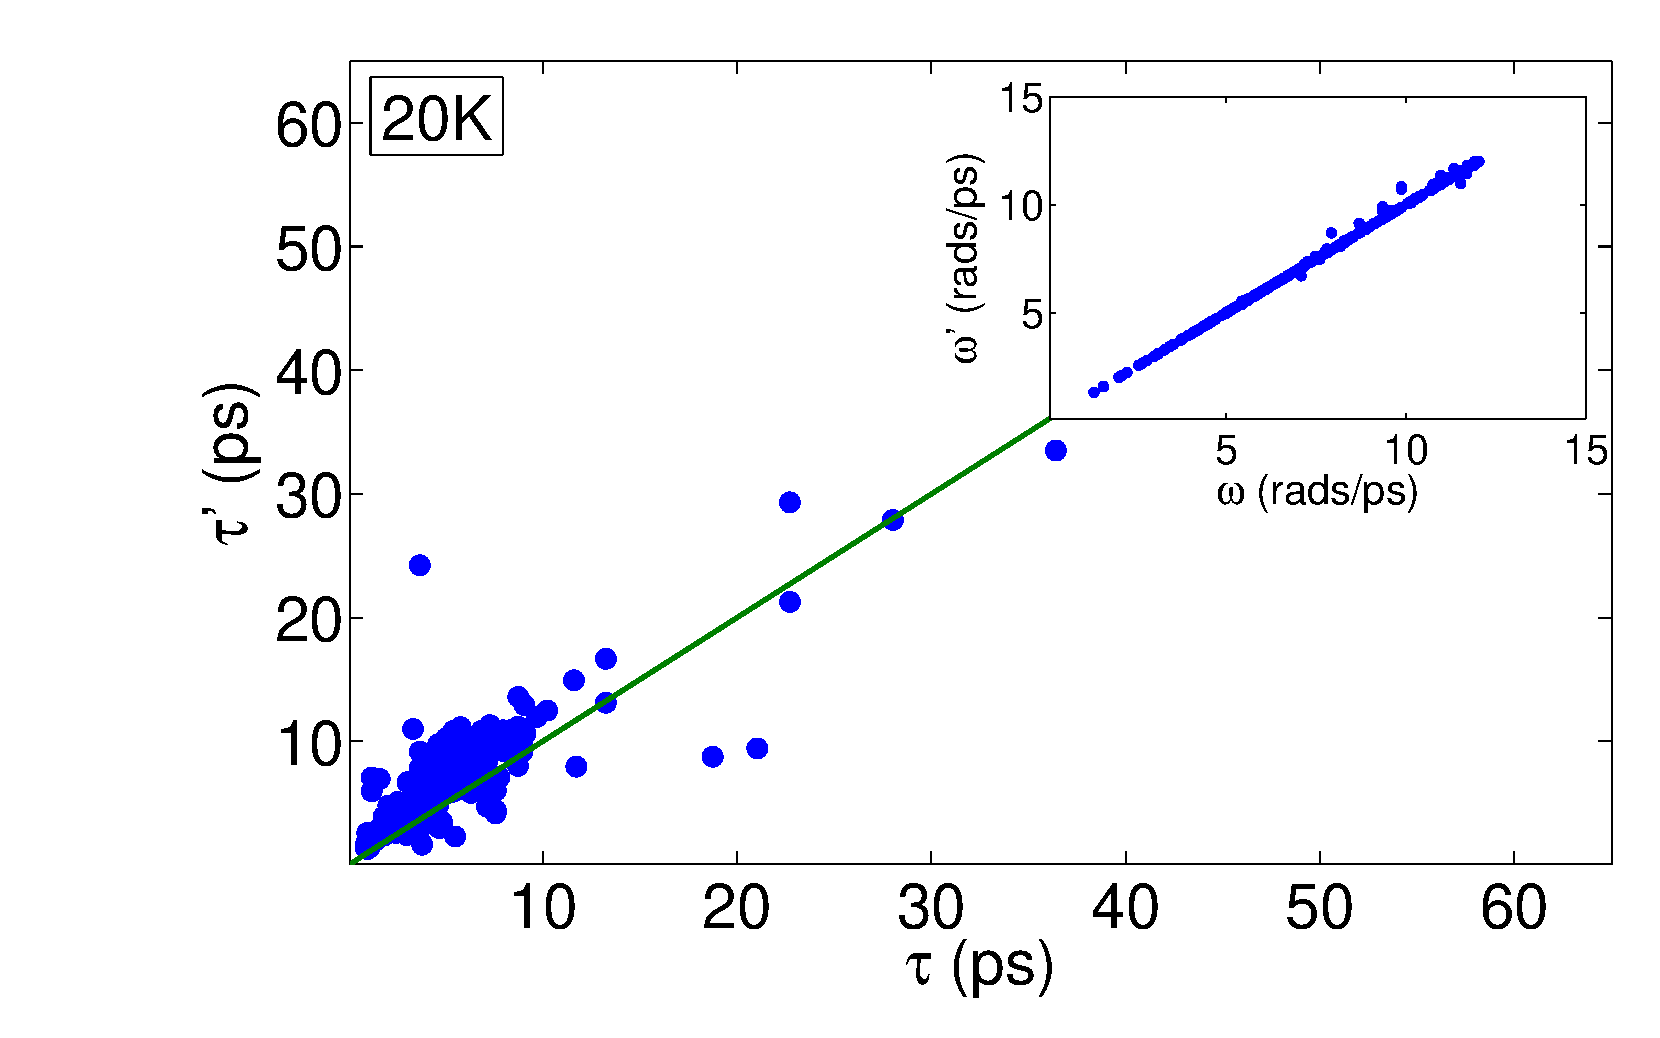
\includegraphics[angle=0,width=80.0mm]{LJ_NMD_SED_20K_2.eps}
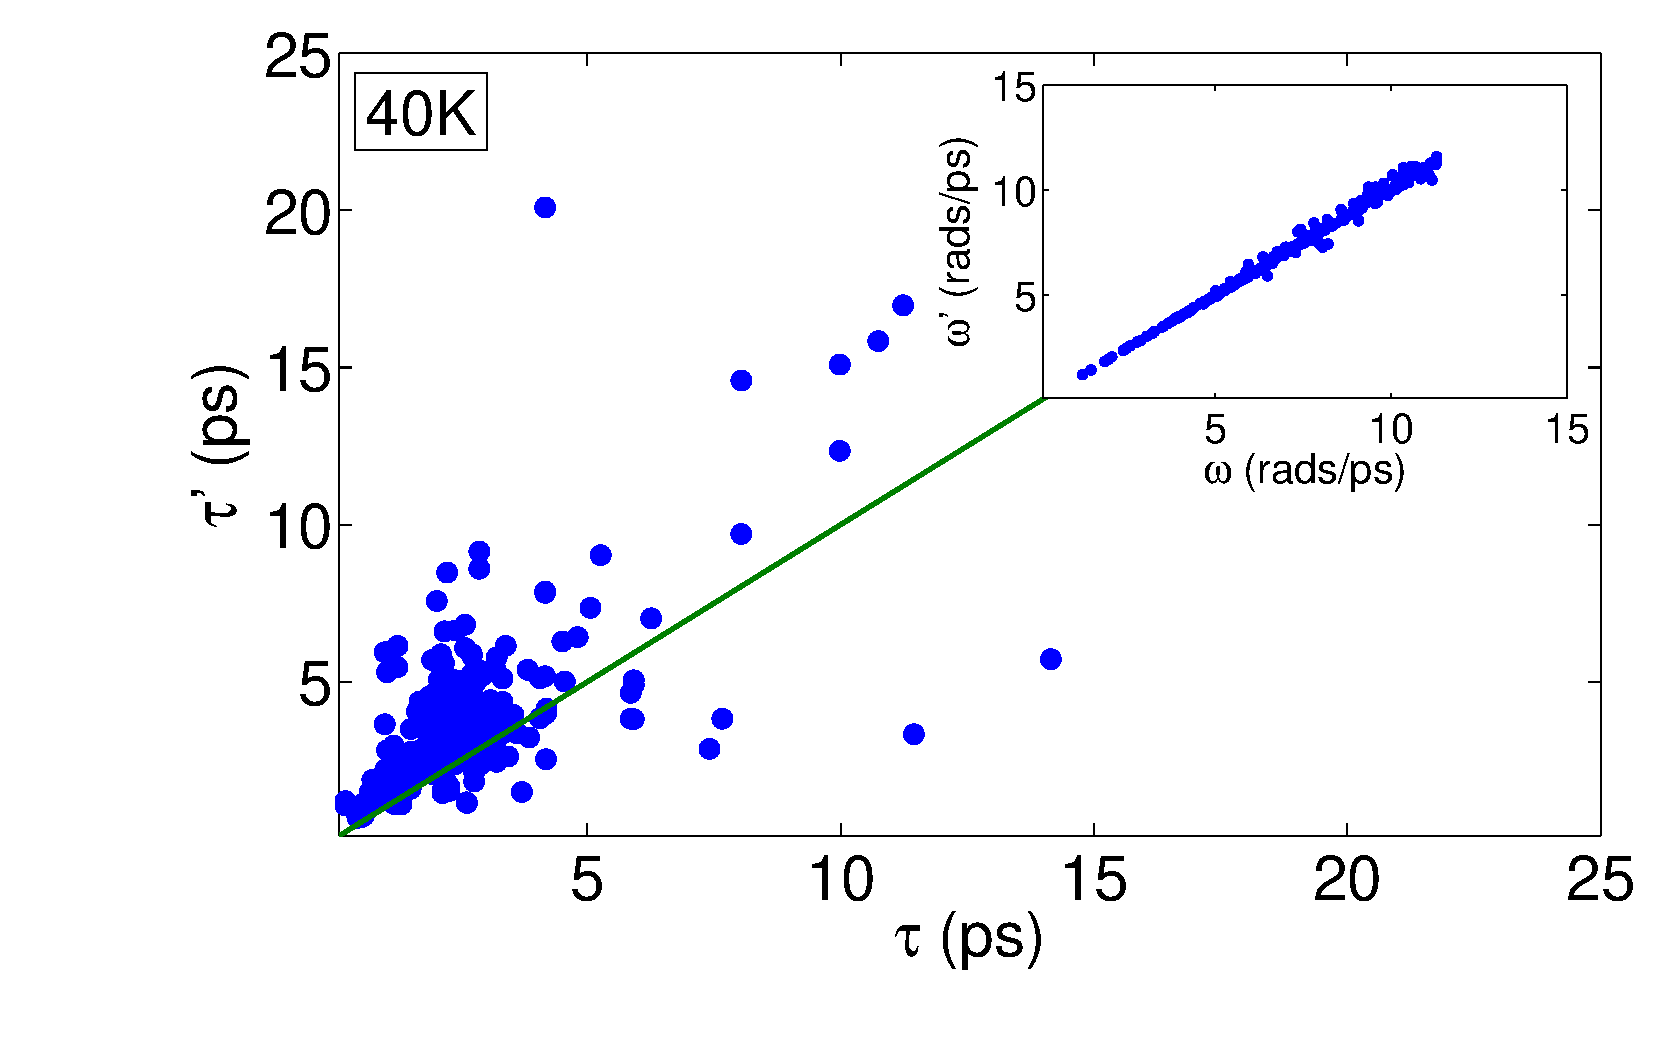
\includegraphics[angle=0,width=80.0mm]{LJ_NMD_SED_40K_2.eps}
\end{center}
\caption{\label{F:FREQ_LIFE_LJ} COMPARISON OF THE PHONON FREQUENCIES AND LIFETIMES MEASURED FROM EQS$.$ \eqref{E:ave_T_w1} ($\omega,\tau$) AND \eqref{Lorentzian_SED} ($\omega^{'},\tau^{'}$) FOR LENNARD-JONES ARGON.}
\end{figure}

\section*{Stillinger-Weber Silicon Case Study}\label{S:Si_Case_study}

We also perform molecular dynamics (MD) simulation to compare the spectral energy calculated for Stillinger-Weber silicon \cite{stillinger1985} at a temperature of $300$K and zero pressure. The Stillinger-Weber system is stiffer (larger phonon group velocities and lifetimes) than Lennard-Jones argon. The MD system consists
of $6\times 6\times 6$ conventional unit cells ($b=8$ atoms) for a total of 1728 atoms.
Using a 0.5 fs timestep, the system is equilibrated for $2^{20}$ time steps before collecting data every $2^5$ time step for $2^{22}$ time steps. The results of five independent simulations (with different initial conditions) are then averaged.

The phonon frequencies and lifetimes have been extracted for all allowed wavevectors in the Brioullin zone (BZ) of the cubic conventional cell using both expressions for the spectral energy and are shown in Fig. \ref{F:FREQ_LIFE_Si}. Like the LJ system, the phonon frequencies can be predicted accurately by Eq$.$ \eqref{Lorentzian_SED} but the lifetimes show large scatter on a mode-by-mode basis.

\begin{figure}
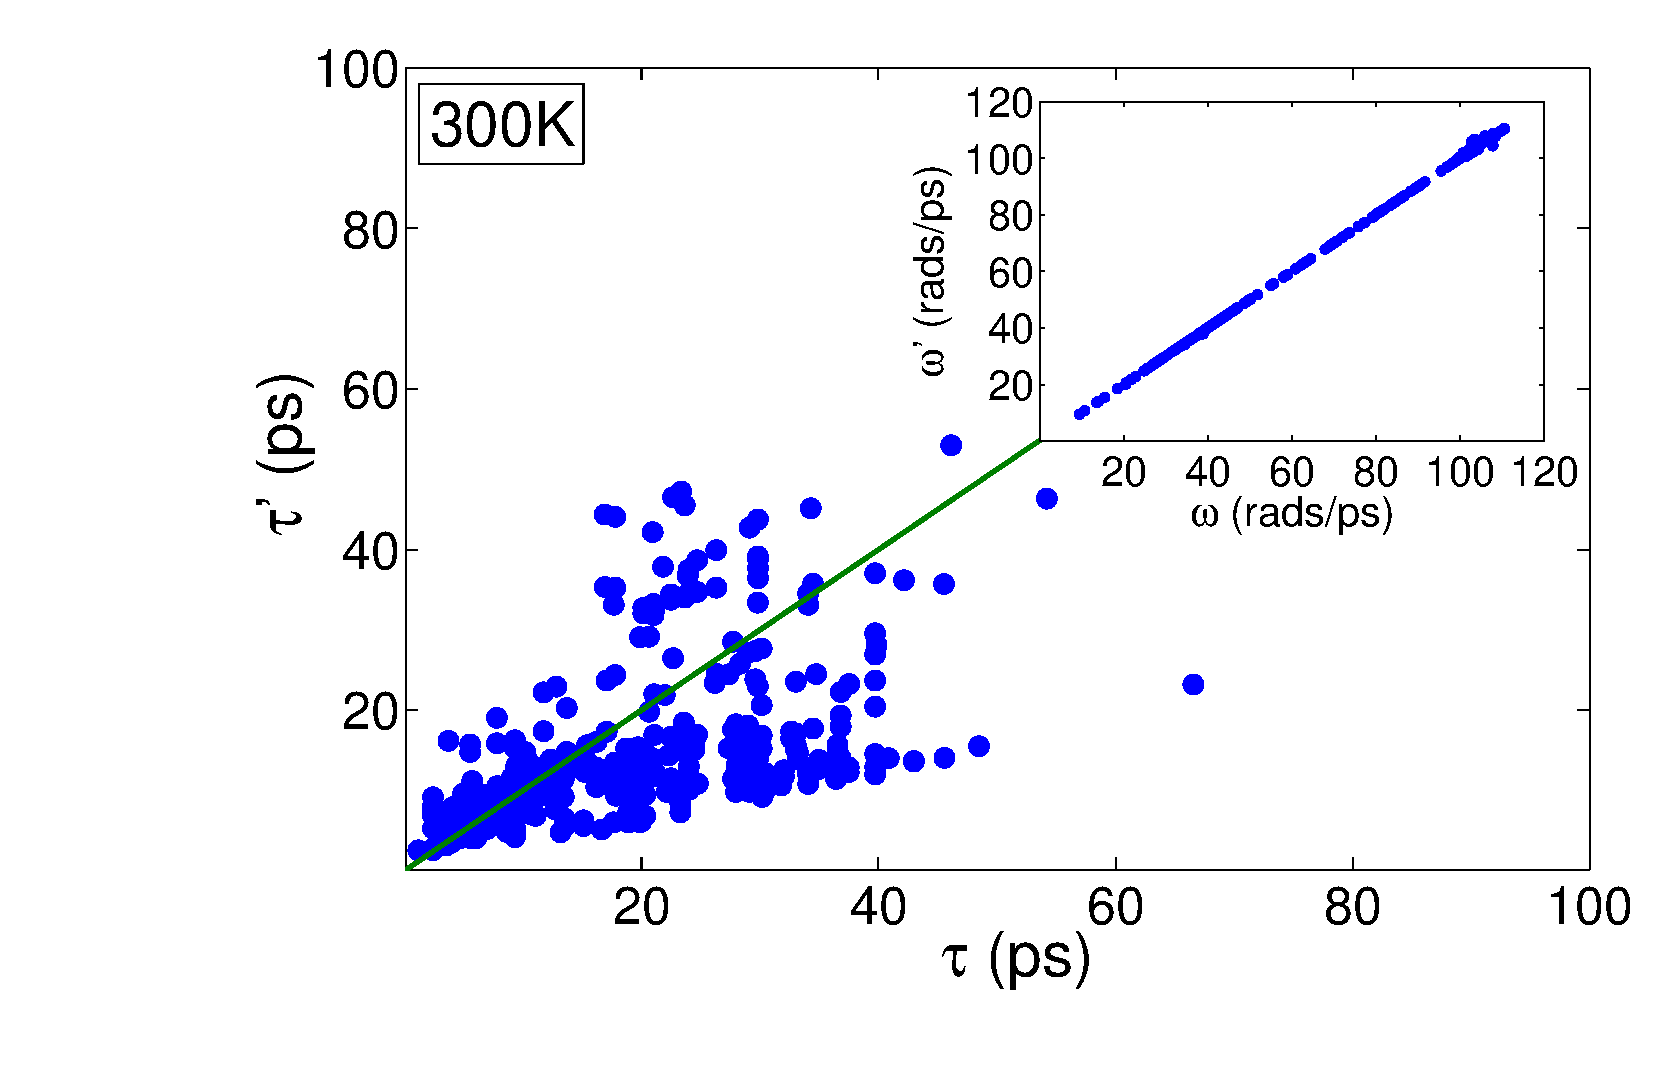
\includegraphics[angle=0,width=80.0mm]{Si_NMD_SED_2.eps}
\caption{\label{F:FREQ_LIFE_Si} COMPARISON OF THE PHONON FREQUENCIES AND LIFETIMES MEASURED FROM EQS$.$ \eqref{E:ave_T_w1} ($\omega,\tau$) AND  \eqref{Lorentzian_SED} ($\omega',\tau'$) FOR STILLINGER-WEBER SILICON.}
\end{figure}

\section*{INTERPRETATION OF PROPOSED ALTERNATIVE PHONON SPECTRAL ENERGY}\label{S:Interpretation}

As demonstrated in the previous sections, Eq. \eqref{Lorentzian_SED} does not represent the total phonon spectal energy as in Eq$.$ \eqref{E:ave_T_w1}. However, Eq. \eqref{Lorentzian_SED} does contain information about the phonon frequencies.  Under the harmonic approximation (or as the temperature approaches $0$K), the phonons are non-interacting and have no transient response, i.e.
\begin{equation}\label{E:qdot_A_SS}
\dot{q}\kvt = \dot{q}_{SS}\kvt = i\omega_0\kv\left\{C_1\kv\exp[i\omega_0\kv t]-C_2\kv\exp[-i\omega_0\kv t]\right\}.
\end{equation}
Inserting this expression into Eq$.$ \eqref{SED} gives
\begin{multline}\label{Delta_SED}
\sum_\alpha^3 \sum_b^n m_b \left| \sum_l^N  \int_{-\infty}^{\infty} \dot{u}_{\alpha}\lbt \EXP{i\pmb{\kappa}\cdot\mathbf{r}_0\ab{l}{0}-i\omega t} dt \right|^2 =
\\ \sum_\alpha^3 \sum_b^n\left| \frac{m_b^{3/2}}{\sqrt{N}} \sum_l^N \sum_{\nu}^{3n}  D\kvba \EXP{i\pmb{\kappa}\cdot\mathbf{r}_0\ab{l}{0}} \delta( \omega_0\kv - \omega) \right|^2 ,
\end{multline}
where $D\kvba = i\sqrt{2\pi} \omega_0\kv C_1\kv e^*\kvba$ and $\delta$ is the Dirac function. Thus, at $0$K, Eq$.$ \eqref{Lorentzian_SED} is a superposition of delta peaks at the phonon frequencies $\omega_0\kv$. This expression is similar to the power spectrum of the mass weighted velocity autocorrelation function \cite{dove1993}, which is equal to the phonon density of states (DOS). Here, Eq$.$ \eqref{Lorentzian_SED} can be interpreted as the phonon DOS for a given wavevector. At finite temperature the phonon spectral energy will broaden into Lorentizain peaks as in Eq$.$ \eqref{E:Lorentzian_NMD}. The broadening of Eq$.$ \eqref{Delta_SED} is undetermined without a knowledge of the phonon mode eigenvectors $e^*\kvba$. Thus, while Eq$.$ \eqref{Lorentzian_SED} can measure the phonon frequencies $\omega_0\kv$, it cannot accurately measure the phonon lifetimes $\tau\kv$.

\section*{SUMMARY}\label{S:Summary}

In this paper, we derived the spectral energy density from the normal mode decomposition and its relation to the phonon frequencies and relaxation
times. We then presented an alternative formulation to the phonon spectral energy which does not require knowledge of the phonon properties {\em a priori}.  Because of this, the alternative formulation does not represent the phonon spectral energy but does represent the phonon frequencies as the temperature approaches $0$K.

We then calculated the spectral energy density for Lennard-Jones argon and Stilinger-Weber silicon using Eqs$.$ \eqref{E:ave_T_w1} and \eqref{Lorentzian_SED}. The phonon frequencies and
relaxation times are measured from the spectral curves at various temperatures as shown in Fig$.$ \ref{F:FREQ_LIFE_LJ} and \ref{F:FREQ_LIFE_Si}. The
frequencies are in excellent agreement between these two SED methods, while the lifetimes show large scatter. This result is not due to the low temperature approximations inherent in LD techniques
\cite{turney2009a}. The phonon spectral energy density $\Phi$ is well-defined theoretically,\cite{dove1993,wallace1972} while $\Phi'$ does not properly map the phonon energies since it is missing the phonon eigenvector. We deduce that this is the reason $\Phi'$ cannot accurately predict the phonon lifetimes. We recommend that $\Phi'$ be used only for measuring phonon dispersion, as in the original formulation \cite{marayuma2003}.

%%%%%%%%%%%%%%%%%%%%%%%%%%%%%%%%%%%%%%%%%%%%%%%%%%%%%%%%%
\begin{acknowledgment}
This work is supported by AFOSR award FA95501010098.
\end{acknowledgment}

%%%%%%%%%%%%%%%%%%%%%%%%%%%%%%%%%%%%%%%%%%%%%%%%%%%%%%%%%
\bibliographystyle{asmems4}

\bibliography{jan10}

%%%%%%%%%%%%%%%%%%%%%%%%%%%%%%%%%%%%%%%%%%%%%%%%%%%%%%%%%

\end{document}
